\section{Construct adjacency matrices from connectivity data [10 points]}
For this exercise the goal was to read the csv file of each graph and create a sparse adjacency matrix which must symmetric and sparse.
To ensure the first property  we applied the code seen in Listing \ref{lst:sym}, where we check if the matrix is symmetric and if not do the necessary adjustment.
To ensure the second property we use the \texttt{sparse} function to create a sparse matrix.
\begin{lstlisting}[language=Matlab, caption=Ensure symmetric property, label=lst:sym]
W = sparse(from,to, 1, nodes, nodes);
if ~issymmetric(W)
	W = (W+W')/2;
	disp('The adjacency matrix has been symmetrized.');
end
\end{lstlisting}

\begin{figure}[H]
	\centering
	\begin{subfigure}{0.5\textwidth}
		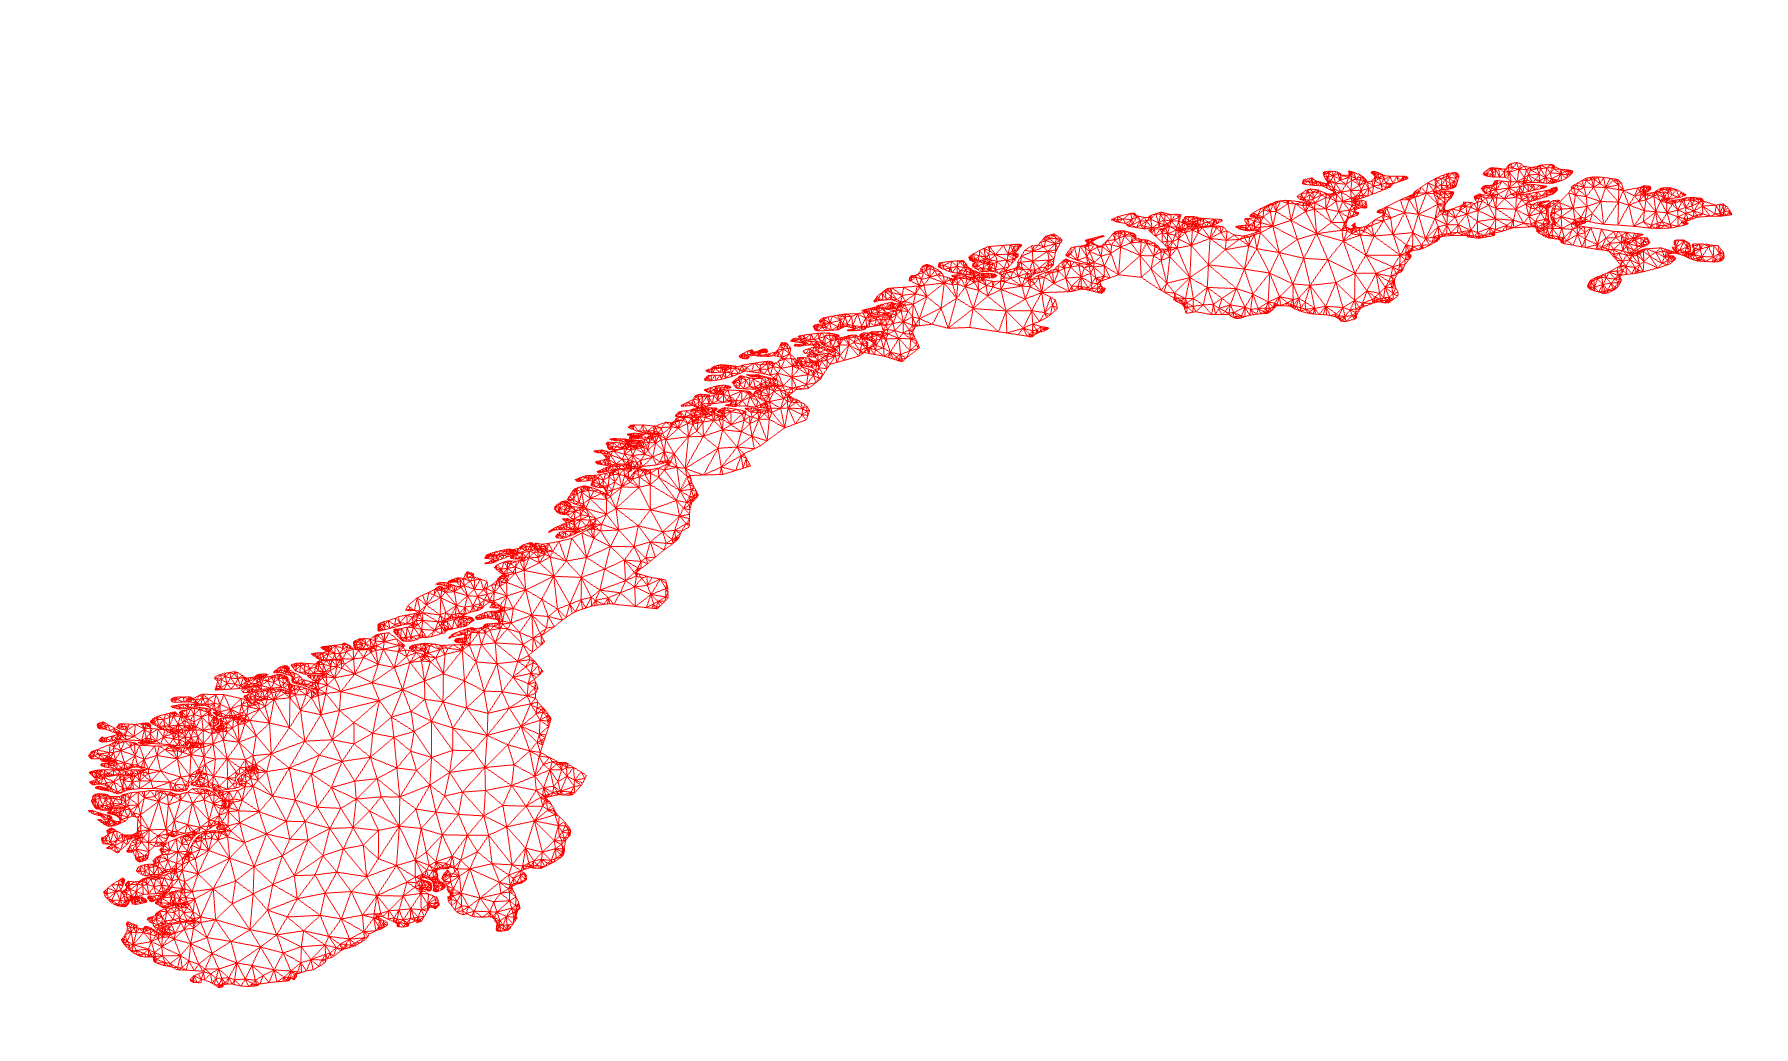
\includegraphics[width=\textwidth]{./media/norway.png}
		\caption{Norway}
		\label{fig:no}
	\end{subfigure}%
    ~
	\begin{subfigure}{0.5\textwidth}
		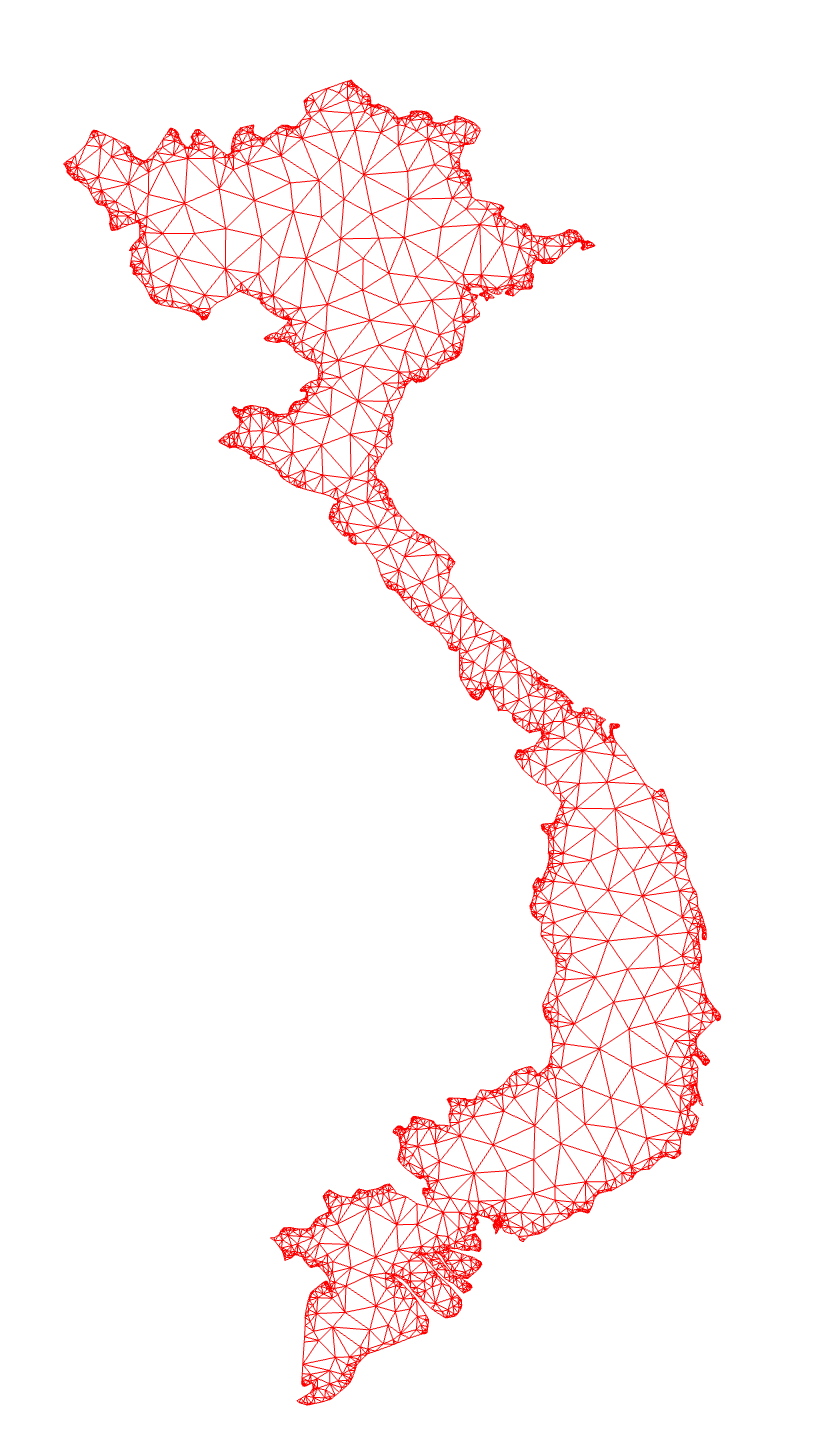
\includegraphics[width=0.5\textwidth]{./media/vietnam.png}
		\caption{Vietnam}
		\label{fig:viet}
	\end{subfigure}
	\caption{Country graphs}
	\label{fig:countries}
\end{figure}
After creating the adjacency matrix we save it and the coordinates matrix in folder \texttt{./Datasets/Countries\_Mat}. As the final step we load the matrices for Norway and Vietnam and visualize it with the provided \texttt{gplotg} function. The resulting graphs can be seen in Figure \ref{fig:countries}.

